\chapter{Methodology}
\label{Chapter4}
\lhead{Chapter 4. \emph{Methodology}}
\todo{Describe implementation details}
In this section we are going to discuss the different classes we used to implmeent our solution.

We have used Python's latest version 3.10 on VS Code.
\newpage

\tikzset{class/.style={rectangle, draw=green!60, fill=green!5, very thick, minimum size=20},
    method/.style={rectangle, draw=yellow!60, fill=yellow!5, very thick, minimum size=20},
    attributes/.style={rectangle, draw=blue!60, fill=blue!5, very thick, minimum size=20},
    instance/.style={rectangle, draw=orange!60, fill=orange!5, very thick, minimum size=20}
}

\newpage
\section{Monte Carlo Tree Search}

\subsection{Generalisation}

The Monte Carlo Tree Search algorithm can be summarised on Figure \ref{fig:Flow MCTS}:
\begin{figure}[!ht]
    \centering
    \begin{tikzpicture}[
            startstop/.style={ellipse, minimum width=3cm, minimum height=1cm, text centered, draw=black},
            process/.style={rectangle, minimum width=3cm, minimum height=1cm, text centered, draw=black},
            decision/.style={rectangle, minimum width=3cm, minimum height=1cm, text centered, draw=black, decorate, decoration={zigzag,segment length=2,amplitude=1}},
            arrow/.style={thick,->,>=stealth},
            node distance=2cm
        ]

        \node (start) [startstop] {start};
        \node (current) [process, below of=start] {Node = $S_0$};
        \node (decision1) [decision, below of=current, yshift=-0.5cm] {is Node a leaf node?};
        \node (ucb1) [process, below of=decision1, yshift=-1cm, align=center] {Node = child node of Node \\ that minimises the \\ chosen selection function};
        \node (decision2) [decision, right of=decision1, xshift=4cm] {Node has never been visited};
        \node (expand) [process, below of=decision2, yshift=-1cm, align=center] {For each available action\\ from Node, add a new \\ state to the tree};
        \node (firstChild) [process, below of=expand] {Node = random new child node};
        \node (rollout1) [process, below of=firstChild] {ROLLOUT - simulation policy};
        \node (rollout2) [process, above of=decision2] {ROLLOUT - simulation policy};

        \draw [arrow] (start) -- (current);
        \draw [arrow] (current) -- (decision1);
        \draw [arrow] (decision1) -- node[anchor=east] {no} (ucb1);
        \draw [arrow] (ucb1) -- (decision1);
        \draw [arrow] (decision1) -- node[anchor=south] {yes} (decision2);
        \draw [arrow] (decision2) -- node[anchor=east] {no} (expand);
        \draw [arrow] (decision2) -- node[anchor=east] {yes} (rollout2);
        \draw [arrow] (expand) -- (firstChild);
        \draw [arrow] (ucb1.west) -- ++(-1,0) |- (decision1.west);
        \draw [arrow] (firstChild) -- (rollout1);

    \end{tikzpicture}
    \caption{Flow MCTS}
    \label{fig:Flow MCTS}
\end{figure}

In every iteration of this algorithm - there are four different phases:

\begin{enumerate}
    \item \textbf{Selection:} Starting from the root node (the starting airport $S_{i0}$ for $I_{i}$), select successive child nodes (airports that are in unvisited areas) until a leaf node (the airport in the initial area - not necessarly the starting airport) is reached. Use the Upper Confidence Bound for Trees (UCB1) formula to balance exploration and exploitation.

          \begin{equation}
              UCB1(S^{n_i,t_i}_i) = \bar{V_i} + c \sqrt{\frac{\ln N}{n_i}}
          \end{equation}

          where:
          \begin{itemize}
              \item $\bar{V_i} = \frac{t_i}{n_i}$ is the average value of the node.
              \item $c$ is the exploration parameter - theoretically equal to $\sqrt2$; in practice it is chosen empirically.
              \item $n_i$ is the number of times node $i$ has been visited.
              \item $N$ is the total number of visits for the root node.
          \end{itemize}

          As oppose to the example in Section \ref{Example}, here we are going to select node with the lowest $UCB1$ value because we want to minimise the overall traveler's cost.

    \item \textbf{Expansion:} If the selected node is not a terminal node, expand the tree by adding all possible child nodes.

    \item \textbf{Simulation:} From the newly added node, perform a simulation (for example take random available flights from these nodes to a terminal node).

    \item \textbf{Backpropagation:} Update the values of the nodes along the path from the newly added node to the root based on the result of the simulation.

          \begin{equation}
              \mathcal{B}(S^{n_i,t_i}_i) = S^{n_i+1,t_i+\mathcal{R}(S^{n_i,t_i}_i)}_i
          \end{equation}

          where $\mathcal{R}(S^{n_i,t_i}_i)$ is the result of the simulation starting from node $S^{n_i,t_i}_i$.
\end{enumerate}


\newpage
\subsubsection{Data Preprocessing}

In order to implement our solution, the first thing to implement was a data\_preprocessing \tikz[baseline=(class.base)]{\node[class] (class) {class};}. All our Python code is oriented-object programmed. We have represented our class on Figure \ref{fig:data_preprocessing_class}.
The input is an \tikz[baseline=(instance.base)]{\node[instance] (instance) {instance};} $I_i$, as defined in Chapter \ref{Chapter3}:

\begin{figure}[!ht]
    \centering
    \begin{tikzpicture}[
            class/.style={rectangle, draw=green!60, fill=green!5, very thick, minimum size=40},
            methods/.style={rectangle, draw=yellow!60, fill=yellow!5, very thick, minimum size=40},
            attributes/.style={rectangle, draw=blue!60, fill=blue!5, very thick, minimum size=40},
            instance/.style={rectangle, draw=orange!60, fill=orange!5, very thick, minimum size=40}
        ]

        %Nodes  
        \node[instance]          (Instance){$I_i = (N_i, S_{i0}, A_{i}, F_{i})$};
        \node[class]             (Class)[below=of Instance]{data preprocessing};

        \node[attributes, left=of  Class , yshift=-40] (Attr1) {$N_i$};
        \node[attributes, left=of  Class , yshift=-90] (Attr2) {$S_{i0}$};
        \node[attributes, left=of  Class , yshift=-140] (Attr3) {flights\_by\_day\_dict};
        \node[attributes, left=of  Class, yshift=-190] (Attr4) {airports\_by\_area};
        \node[attributes, left=of  Class, yshift=-240] (Attr5) {area\_by\_airport};
        %\node[methods, left=of Class, yshift=-290, align=center] (Meth10) {flights\_from\_airport\_at\_a\_\\specific\_day\_with\_previous\_areas};
        \node[methods, left=of Class, yshift=-290, align=center] (Meth10) {specific\_flights};


        \node[methods, right=of  Class, yshift=-40] (Meth1) {read\_file};
        \node[methods, right=of  Class, yshift=-90] (Meth2) {flights\_by\_day};
        \node[methods, right=of  Class, yshift=-140] (Meth3) {flights\_from\_airport};
        \node[methods, right=of  Class, yshift=-190] (Meth4) {associated\_area\_to\_airport};
        \node[methods, right=of  Class, yshift=-240] (Meth5) {get\_cost};
        \node[methods, right=of  Class, yshift=-290] (Meth6) {get\_airports\_by\_areas};
        \node[methods, below=of  Class, yshift=-220] (Meth7) {remove\_duplicate};

        %Lines
        \draw[->, very thick] (Instance.south)  to node[midway, right] {} (Class.north);

        \draw[->] (Class.south) to[out=180, in=0] (Attr1.east);
        \draw[->] (Class.south) to[out=190, in=0] (Attr2.east);
        \draw[->] (Class.south) to[out=200, in=0] (Attr3.east);
        \draw[->] (Class.south) to[out=210, in=0] (Attr4.east);
        \draw[->] (Class.south) to[out=220, in=0] (Attr5.east);

        % Arrows from Class to Methods (right side)
        \draw[->] (Class.south) to[out=0, in=180] (Meth1.west);
        \draw[->] (Class.south) to[out=350, in=180] (Meth2.west);
        \draw[->] (Class.south) to[out=340, in=180] (Meth3.west);
        \draw[->] (Class.south) to[out=330, in=180] (Meth4.west);
        \draw[->] (Class.south) to[out=320, in=180] (Meth5.west);

        \draw[->] (Class.south) to[out=-115, in=30] (Meth10.east);
        \draw[->] (Class.south) to[out=-65, in=150] (Meth6.west);
        \draw[->] (Class.south) to[out=-90, in=90] (Meth7.north);
    \end{tikzpicture}
    \caption{Explanation of the data preprocessing class}
    \label{fig:data_preprocessing_class}
\end{figure}


Different useful \tikz[baseline=(methods.base)]{\node[method] (methods) {methods};} are implemented to compute data preprocessing \tikz[baseline=(attributes.base)]{\node[attributes] (attributes) {attributes};}. For example, remove\_duplicate considers the cheapest flight connections if multiple flight connections between two airports exist at different prices on the same day.
Thanks to the different methods we can then compute data preprocessing's attributes such as flights\_by\_day\_dict that group all the flights by day, airports\_by\_area group all the airports per area.
Other methods are also defined like specific\_flifhts that will be helpful later and gives you all the possible flight connections from a specific airport on a specific day considering the visited\_areas, it hence gives you all the possibles actions from a node.


It is known that Python is relatively slow in terms of computation, so we decided to use as much as possible hasmaps.
Hashmaps allow to retrieve data efficiently based on a key - with a $\mathcal{O}(1)$ in term of time complexity.


\newpage
\subsubsection{Node}
\begin{figure}[h]
    \centering
    \begin{tikzpicture}[
            class/.style={rectangle, draw=green!60, fill=green!5, very thick, minimum size=40},
            methods/.style={rectangle, draw=yellow!60, fill=yellow!5, very thick, minimum size=40},
            attributes/.style={rectangle, draw=blue!60, fill=blue!5, very thick, minimum size=40},
            instance/.style={rectangle, draw=orange!60, fill=orange!5, very thick, minimum size=40}
        ]

        \node[class]             (Class){\phantom{-----}Node\phantom{-----}};

        \node[attributes, left=of  Class , yshift=-40] (Attr1) {state};
        \node[attributes, left=of  Class , yshift=-90] (Attr2) {parent};
        \node[attributes, left=of  Class , yshift=-140] (Attr3) {children};
        \node[attributes, left=of  Class, yshift=-190] (Attr4) {visit\_count};

        \node[methods, right=of  Class, yshift=-40] (Meth1) {add\_child};
        \node[methods, right=of  Class, yshift=-90] (Meth2) {is\_fully\_expanded};
        \node[methods, right=of  Class, yshift=-140] (Meth3) {best\_child};
        \node[methods, right=of  Class, yshift=-190] (Meth4) {update};

        \node[attributes, below=of  Class, yshift=-120] (Meth5) {total\_cost};


        \draw[->] (Class.south) to[out=180, in=0] (Attr1.east);
        \draw[->] (Class.south) to[out=190, in=0] (Attr2.east);
        \draw[->] (Class.south) to[out=200, in=0] (Attr3.east);
        \draw[->] (Class.south) to[out=210, in=0] (Attr4.east);

        \draw[->] (Class.south) to[out=0, in=180] (Meth1.west);
        \draw[->] (Class.south) to[out=350, in=180] (Meth2.west);
        \draw[->] (Class.south) to[out=340, in=180] (Meth3.west);
        \draw[->] (Class.south) to[out=330, in=180] (Meth4.west);

        \draw[->] (Class.south) to[out=-90, in=90] (Meth5.north);

    \end{tikzpicture}
    \caption{Explanation of the Node class}
    \label{fig:node_class}
\end{figure}

As already mentionned during the example, we use Node structure in our algorithm, we hence defined a Node class.
A node has one parent (if it is not the root node) or children(s) (if it is not a leaf node), they also have a number of times they have been visited - visit\_count and the total\_cost.
We also add a state which is a dictionnary where we keep track of the current\_airport and the current\_day, the remaining\_zones we have to visit from this node to end the traveler's journey, the visited\_zones so far, and the total\_cost of the undertaken flight connections that is going to evolve for the simulation and then be backpropagated to the total\_cost of the node if a terminal node is reached.

\newpage
\subsection{Pseudo-code}
\begin{figure}[!ht]
    \centering
    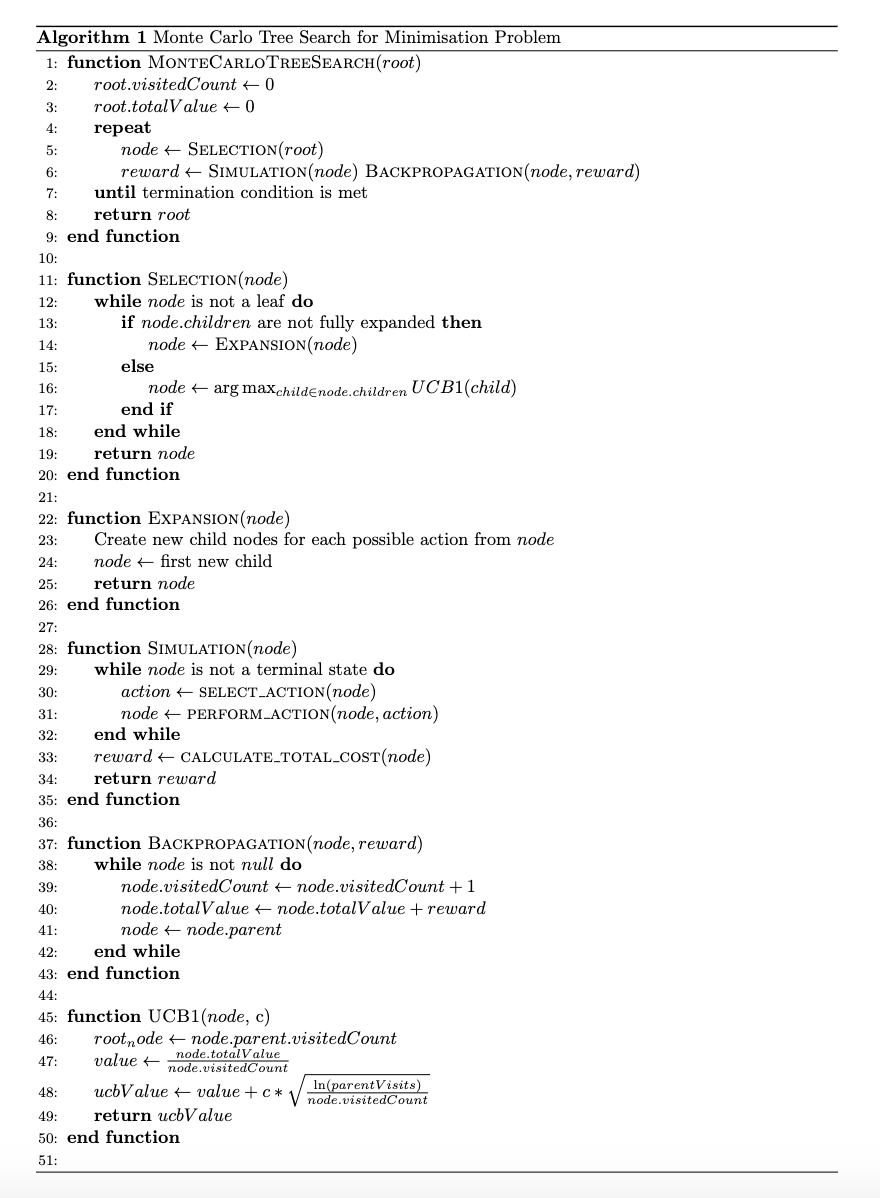
\includegraphics[width=1\textwidth]{Figures/Pseudo code.png}
\end{figure}
\newpage
\subsection{Different policies}
\subsubsection{Selection policy}
Our selection policy is based on
\subsubsection{Simulation policy}


\begin{algorithm}[H]
    \caption{Monte Carlo Tree Search (MCTS)}
    \label{alg:MCTS}
    \begin{algorithmic}[1]
        \STATE Initialize root node with initial state
        \FOR{number of simulations}
        \STATE $node \leftarrow \text{Select}(root)$
        \IF{$node$ is not fully expanded}
        \STATE $node \leftarrow \text{Expand}(node)$
        \ENDIF
        \STATE $cost \leftarrow \text{Simulate}(node)$
        \STATE \text{Backpropagate}($node$, $cost$)
        \ENDFOR
        \RETURN $BestLeafNode$
    \end{algorithmic}
\end{algorithm}


\begin{algorithm}[H]
    \caption{Select Function}
    \label{alg:Select}
    \begin{algorithmic}[1]
        \STATE $currentNode \leftarrow root$
        \WHILE{True}
        \STATE $unvisitedChildren \leftarrow \text{GetUnvisitedChildren}(currentNode)$
        \IF{$unvisitedChildren$ is not empty}
        \STATE \textbf{return} \text{Randomly select from} $unvisitedChildren$
        \ENDIF
        \IF{$currentNode$ has no children}
        \STATE \text{ExpandNode}($currentNode$)
        \IF{$currentNode$ has no children after expansion}
        \STATE \textbf{return} $None$
        \ENDIF
        \STATE \textbf{return} \text{Randomly select from} $currentNode.children$
        \ENDIF
        \STATE $currentNode \leftarrow \text{BestChild}(currentNode)$
        \ENDWHILE
    \end{algorithmic}
\end{algorithm}

\begin{algorithm}[H]
    \caption{Expand Function}
    \label{alg:Expand}
    \begin{algorithmic}[1]
        \STATE $actions \leftarrow \text{PossibleActions}(currentNode.state)$
        \STATE $expansionPolicy \leftarrow \text{GetExpansionPolicy}()$
        \STATE $actions \leftarrow expansionPolicy(actions)$
        \FOR{each $action$ in $actions$}
        \STATE $newState \leftarrow \text{TransitionFunction}(currentNode.state, action)$
        \STATE \text{AddChild}(currentNode, newState)
        \ENDFOR
    \end{algorithmic}
\end{algorithm}

\begin{algorithm}[H]
    \caption{Simulate Function}
    \label{alg:Simulate}
    \begin{algorithmic}[1]
        \STATE $currentSimulationState \leftarrow \text{Copy of } node.state$
        \WHILE{$currentSimulationState.currentDay \neq \text{Number of Areas}$}
        \STATE $actions \leftarrow \text{PossibleActions}(currentSimulationState)$
        \STATE $action \leftarrow \text{SimulationPolicy}(actions)$
        \IF{$action$ is $None$}
        \STATE \textbf{return} $False$
        \ENDIF
        \STATE $currentSimulationState \leftarrow \text{TransitionFunction}(currentSimulationState, action)$
        \ENDWHILE
        \IF{$currentSimulationState.currentDay == \text{Number of Areas}$}
        \STATE $returnFlightActions \leftarrow \text{FlightsToReturn}(currentSimulationState)$
        \IF{$returnFlightActions$ is empty}
        \STATE \textbf{return} $False$
        \ENDIF
        \STATE $action \leftarrow \text{SimulationPolicy}(returnFlightActions)$
        \STATE $currentSimulationState \leftarrow \text{TransitionFunction}(currentSimulationState, action)$
        \ENDIF
        \RETURN $currentSimulationState.totalCost$
    \end{algorithmic}
\end{algorithm}

\begin{algorithm}[H]
    \caption{Backpropagate Function}
    \label{alg:Backpropagate}
    \begin{algorithmic}[1]
        \WHILE{$node$ is not $None$}
        \STATE $node.update(cost)$
        \STATE $node \leftarrow node.parent$
        \ENDWHILE
    \end{algorithmic}
\end{algorithm}

\begin{algorithm}[H]
    \caption{Transition Function}
    \label{alg:TransitionFunction}
    \begin{algorithmic}[1]
        \STATE $newState \leftarrow \text{Copy of } state$
        \STATE $newState.currentDay \leftarrow state.currentDay + 1$
        \STATE $newState.currentAirport \leftarrow action[0]$
        \STATE $newState.totalCost \leftarrow state.totalCost + action[1]$
        \STATE \text{Update}($newState.path$, $newState.currentAirport$)
        \STATE \text{RemoveVisitedZone}($newState.remainingZones$, $newState.currentAirport$)
        \STATE \text{AddVisitedZone}($newState.visitedZones$, $newState.currentAirport$)
        \RETURN $newState$
    \end{algorithmic}
\end{algorithm}

\subsection{selection policies} % (fold)
\label{sub:selection policies}

% subsection selection policies (end)

\begin{algorithm}[H]
    \caption{UCB Selection}
    \label{alg:UCB}
    \begin{algorithmic}[1]
        \STATE $\epsilon \leftarrow 0$
        \STATE $visitedChildren \leftarrow \text{Children with } visitCount > 0$
        \STATE $sortedChildren \leftarrow \text{Sort } visitedChildren \text{ by } \frac{totalCost}{visitCount + \epsilon}$
        \STATE $scores \leftarrow \text{Assign ranks to sortedChildren}$
        \STATE $totalScores \leftarrow \sum scores$
        \STATE $normalizedScore(child) \leftarrow \frac{scores[child]}{totalScores}$
        \STATE $choicesWeights \leftarrow \left[ normalizedScore(child) + cParam \times \sqrt{\frac{2 \times \log(visitCount)}{child.visitCount + \epsilon}} \text{ for each child in } visitedChildren \right]$
        \STATE $bestChildNode \leftarrow \text{Child with minimum } choicesWeights$
        \RETURN $bestChildNode$
    \end{algorithmic}
\end{algorithm}

\begin{algorithm}[H]
    \caption{SP Selection}
    \label{alg:SP}
    \begin{algorithmic}[1]
        \STATE $visitedChildren \leftarrow \text{Children with } visitCount > 0$
        \STATE $D \leftarrow 1$
        \STATE $spMctsScore(child) \leftarrow \text{meanCost} - cp \times \text{possibleDeviation}$
        \STATE $choicesWeights \leftarrow \left[ spMctsScore(child) \text{ for each child in } visitedChildren \right]$
        \STATE $bestChildNode \leftarrow \text{Child with minimum } choicesWeights$
        \RETURN $bestChildNode$
    \end{algorithmic}
\end{algorithm}

\begin{algorithm}[H]
    \caption{Bayesian UCT Selection}
    \label{alg:Bayesian}
    \begin{algorithmic}[1]
        \STATE $visitedChildren \leftarrow \text{Children with } visitCount > 0$
        \STATE $N \leftarrow visitCount$
        \STATE $useVariance \leftarrow \text{True or False depending on the formula}$
        \STATE $bayesianUctScore(child) \leftarrow meanCost + explorationTerm$
        \STATE $choicesWeights \leftarrow \left[ bayesianUctScore(child, useVariance) \text{ for each child in } visitedChildren \right]$
        \STATE $bestChildNode \leftarrow \text{Child with minimum } choicesWeights$
        \RETURN $bestChildNode$
    \end{algorithmic}
\end{algorithm}

\begin{algorithm}[H]
    \caption{UCB1-Tuned Selection}
    \label{alg:UCB1_tuned}
    \begin{algorithmic}[1]
        \STATE $visitedChildren \leftarrow \text{Children with } visitCount > 0$
        \STATE $ucb1TunedScore(child) \leftarrow meanCost + cParam \times \sqrt{\left(\frac{\log(visitCount)}{child.visitCount}\right) \times \min\left(0.25, variance + \sqrt{\frac{2 \times \log(visitCount)}{child.visitCount}}\right)}$
        \STATE $choicesWeights \leftarrow \left[ ucb1TunedScore(child) \text{ for each child in } visitedChildren \right]$
        \STATE $bestChildNode \leftarrow \text{Child with minimum } choicesWeights$
        \RETURN $bestChildNode$
    \end{algorithmic}
\end{algorithm}